%%%%%%%%%%%%%%%%%%%%%%%%%%%%%%%%%%% CABECALHO %%%%%%%%%%%%%%%%%%%%%%%%%%%%%%%%%%%
\documentclass[a4paper]{abntex2}

\usepackage[utf8]{inputenc}
\usepackage{csquotes}
\usepackage[brazil]{babel}
\usepackage[T1]{fontenc}
\usepackage{xcolor,graphicx}
\usepackage[all,defaultlines=2]{nowidow}
\usepackage[multiple]{footmisc}
\usepackage{enumitem}
\usepackage{fmtcount}
\usepackage{multirow}
\usepackage[backend=bibtex,backref=true]{biblatex}
\bibliography{projeto}
\hypersetup{
	colorlinks=true,
	urlcolor=blue,
	linkcolor=black,
	citecolor=red
}


\author{Igor~Santos\\
	Universidade Est\'acio de S\'a\\
	Rio de Janeiro, RJ\\
	\texttt{igorsantos07+conf@gmail.com}
}
\title{Projeto~de~TCC\\BitCongresso}

\makeindex
\begin{document}
\pagenumbering{gobble}
\maketitle

%%%%%%%%%%%%%%%%%%%%%%%%%%%%%%%%%%%%%%%% INICIO %%%%%%%%%%%%%%%%%%%%%%%%%%%%%%%%%%%%%%%%

\chapter*{Prefácio}
\section*{Definições usadas neste documento}
Para fins de comunicação, as seguintes palavras são tidas como sinônimo, exceto quando especificado o contrário -- na seção \ref{sec:eventos} explicaremos os conceitos envolvidos mais a fundo:
\begin{itemize}
	\item Conferência
	\item Congresso
	\item Evento
\end{itemize}
\newpage

\pagenumbering{arabic}
\tableofcontents

\chapter{Proposta do Projeto de TCC}

%%%%%%%%%%%%%%%%%%%%%%%%%%%%%%%%%%%%%%%%%%%%%%%%%%%%%%%%%%%%%%%%%%%%%%%%%%%%%%%%%%%%%%%%%
\section{O Projeto}

É notável a dificuldade que conferencistas possuem, muitas das vezes, em obter informações atualizadas sobre as conferências das quais participarão ou estão participando naquele momento. Esta opinião foi compartilhada por diversas pessoas informalmente consultadas.

Por exemplo, muitas vezes são entregues panfletos ou cartões com a programação, mas esse tipo de objeto frequentemente se perde ou se danifica no decorrer do dia. Sem contar as possíveis alterações de última hora, o que torna a grade distribuída alvo de rabiscos e anotações. Invariavelmente, \emph{slots} de programação indefinida (comum em mesas-redondas ou \emph{lightning talks}\footnotemark) levam o conferencista a se deslocar até o lugar para descobrir se valerá a pena assistir ou não -- ou simplesmente não atender ao \emph{slot}.

Partindo destas premissas, o objetivo do Projeto é criar um aplicativo móvel que permita aos usuários obterem as diversas informações referentes ao evento do qual participam, em tempo real. Informações como: a liberação da grade de programação, atualizações e mudanças da mesma; dados de contato dos palestrantes; detalhes sobre o processo e valores das inscrições; localização e como chegar ao local; comércio e atrações da região; notícias e novidades sobre a conferência em geral. Este aplicativo teria um backend facilmente acessível, onde os organizadores poderiam inserir tais informações.

\footnotetext{Série de palestras de curta duração, dadas pelos próprios conferencistas}

%%%%%%%%%%%%%%%%%%%%%%%%%%%%%%%%%%%%%%%%%%%%%%%%%%%%%%%%%%%%%%%%%%%%%%%%%%%%%%%%%%%%%%%%%
\subsection*{Opções de nome}

Seguem aqui alguns componentes que podem ser utilizados de inspiração para o nome do sistema:\\

\begin{tabular}{rl|c|c}
\multicolumn{2}{c|}{\textbf{Afixos}} & \textbf{Substantivos} & \textbf{Sugestões} \\\hline
Bit		& Data	& Congresso		& \multirow{6}{6cm}{EvenTime \footnotemark, BitConf, Dataconf, QuickConf, ClickConf, HandyConf} \\\cline{1-3}
Time	& App	& Conferência	& \\\cline{1-3}
Quick	& Fast	& Conf			& \\\cline{1-3}
Rápido	& Veloz	& Evento		& \\\cline{1-3}
Click	& Lite	& Event			& \\\cline{1-3}
\multicolumn{2}{c|}{Handy}	& 		& \\
\end{tabular}
\footnotetext{EvenTime pode soar como \emph{Even+Time}}


%%%%%%%%%%%%%%%%%%%%%%%%%%%%%%%%%%%%%%%%%%%%%%%%%%%%%%%%%%%%%%%%%%%%%%%%%%%%%%%%%%%%%%%%%
\section{Método de Trabalho}



%%%%%%%%%%%%%%%%%%%%%%%%%%%%%%%%%%%%%%%%%%%%%%%%%%%%%%%%%%%%%%%%%%%%%%%%%%%%%%%%%%%%%%%%%
\chapter{A Empresa e o Negócio}


%%%%%%%%%%%%%%%%%%%%%%%%%%%%%%%%%%%%%%%%%%%%%%%%%%%%%%%%%%%%%%%%%%%%%%%%%%%%%%%%%%%%%%%%%
\section{Histórico}

%%%%%%%%%%%%%%%%%%%%%%%%%%%%%%%%%%%%%%%%%%%%%%%%%%%%%%%%%%%%%%%%%%%%%%%%%%%%%%%%%%%%%%%%%
\section{Mercado Consumidor}

\subsection{Os tipos de eventos científicos e tecnológicos}
\label{sec:eventos}
blabla

%%%%%%%%%%%%%%%%%%%%%%%%%%%%%%%%%%%%%%%%%%%%%%%%%%%%%%%%%%%%%%%%%%%%%%%%%%%%%%%%%%%%%%%%%
\section{Concorrência}

%%%%%%%%%%%%%%%%%%%%%%%%%%%%%%%%%%%%%%%%%%%%%%%%%%%%%%%%%%%%%%%%%%%%%%%%%%%%%%%%%%%%%%%%%
\section{Premissas e Restrições ao Projeto}

%%%%%%%%%%%%%%%%%%%%%%%%%%%%%%%%%%%%%%%%%%%%%%%%%%%%%%%%%%%%%%%%%%%%%%%%%%%%%%%%%%%%%%%%%
\chapter{Os Sistemas Atuais}

%%%%%%%%%%%%%%%%%%%%%%%%%%%%%%%%%%%%%%%%%%%%%%%%%%%%%%%%%%%%%%%%%%%%%%%%%%%%%%%%%%%%%%%%%
\section{Principais Concorrentes}


%%%%%%%%%%%%%%%%%%%%%%%%%%%%%%%%%%%%%%%%%%%%%%%%%%%%%%%%%%%%%%%%%%%%%%%%%%%%%%%%%%%%%%%%%
\section{Outros Sistemas}

%%%%%%%%%%%%%%%%%%%%%%%%%%%%%%%%%%%%%%%%%%%%%%%%%%%%%%%%%%%%%%%%%%%%%%%%%%%%%%%%%%%%%%%%%
\section{Motivações para o Novo Sistema}

%%%%%%%%%%%%%%%%%%%%%%%%%%%%%%%%%%%%%%%%%%%%%%%%%%%%%%%%%%%%%%%%%%%%%%%%%%%%%%%%%%%%%%%%%
\subsection{Problemas dos Sistemas Atuais}

%%%%%%%%%%%%%%%%%%%%%%%%%%%%%%%%%%%%%%%%%%%%%%%%%%%%%%%%%%%%%%%%%%%%%%%%%%%%%%%%%%%%%%%%%
\subsection{Situação Desejada}

%%%%%%%%%%%%%%%%%%%%%%%%%%%%%%%%%%%%%%%%%%%%%%%%%%%%%%%%%%%%%%%%%%%%%%%%%%%%%%%%%%%%%%%%%
\chapter{Proposta Preliminar de Sistema}

%%%%%%%%%%%%%%%%%%%%%%%%%%%%%%%%%%%%%%%%%%%%%%%%%%%%%%%%%%%%%%%%%%%%%%%%%%%%%%%%%%%%%%%%%
\section{Requisitos do sistema}

%%%%%%%%%%%%%%%%%%%%%%%%%%%%%%%%%%%%%%%%%%%%%%%%%%%%%%%%%%%%%%%%%%%%%%%%%%%%%%%%%%%%%%%%%
\section{Método de monetização}

%%%%%%%%%%%%%%%%%%%%%%%%%%%%%%%%%%%%%%%%%%%%%%%%%%%%%%%%%%%%%%%%%%%%%%%%%%%%%%%%%%%%%%%%%
\section{Tecnologias utilizadas}



\subsection{Topologia}
Conforme citado acima, o \emph{Parse.com} é bem eficiente e focado no que projetos como o nosso demandam. Portanto, é provável que todo o ecossistema por trás de nosso desenvolvimento seja baseado em seus serviços. A partir daí fica claro o motivo da simplicidade da topologia que vamos adotar, visto que a comunicação não terá intermediários. Ela ocorrerá dos desenvolvedores ao Parse, do Parse aos dispositivos, e deles aos clientes do produto: os responsáveis adicionarão lógica e estrutura, outros analisarão os dados coletados, e tais informações serão fornecidas de forma eficiente aos aparelhos conectados.

\begin{figure}[h!]
\centering
	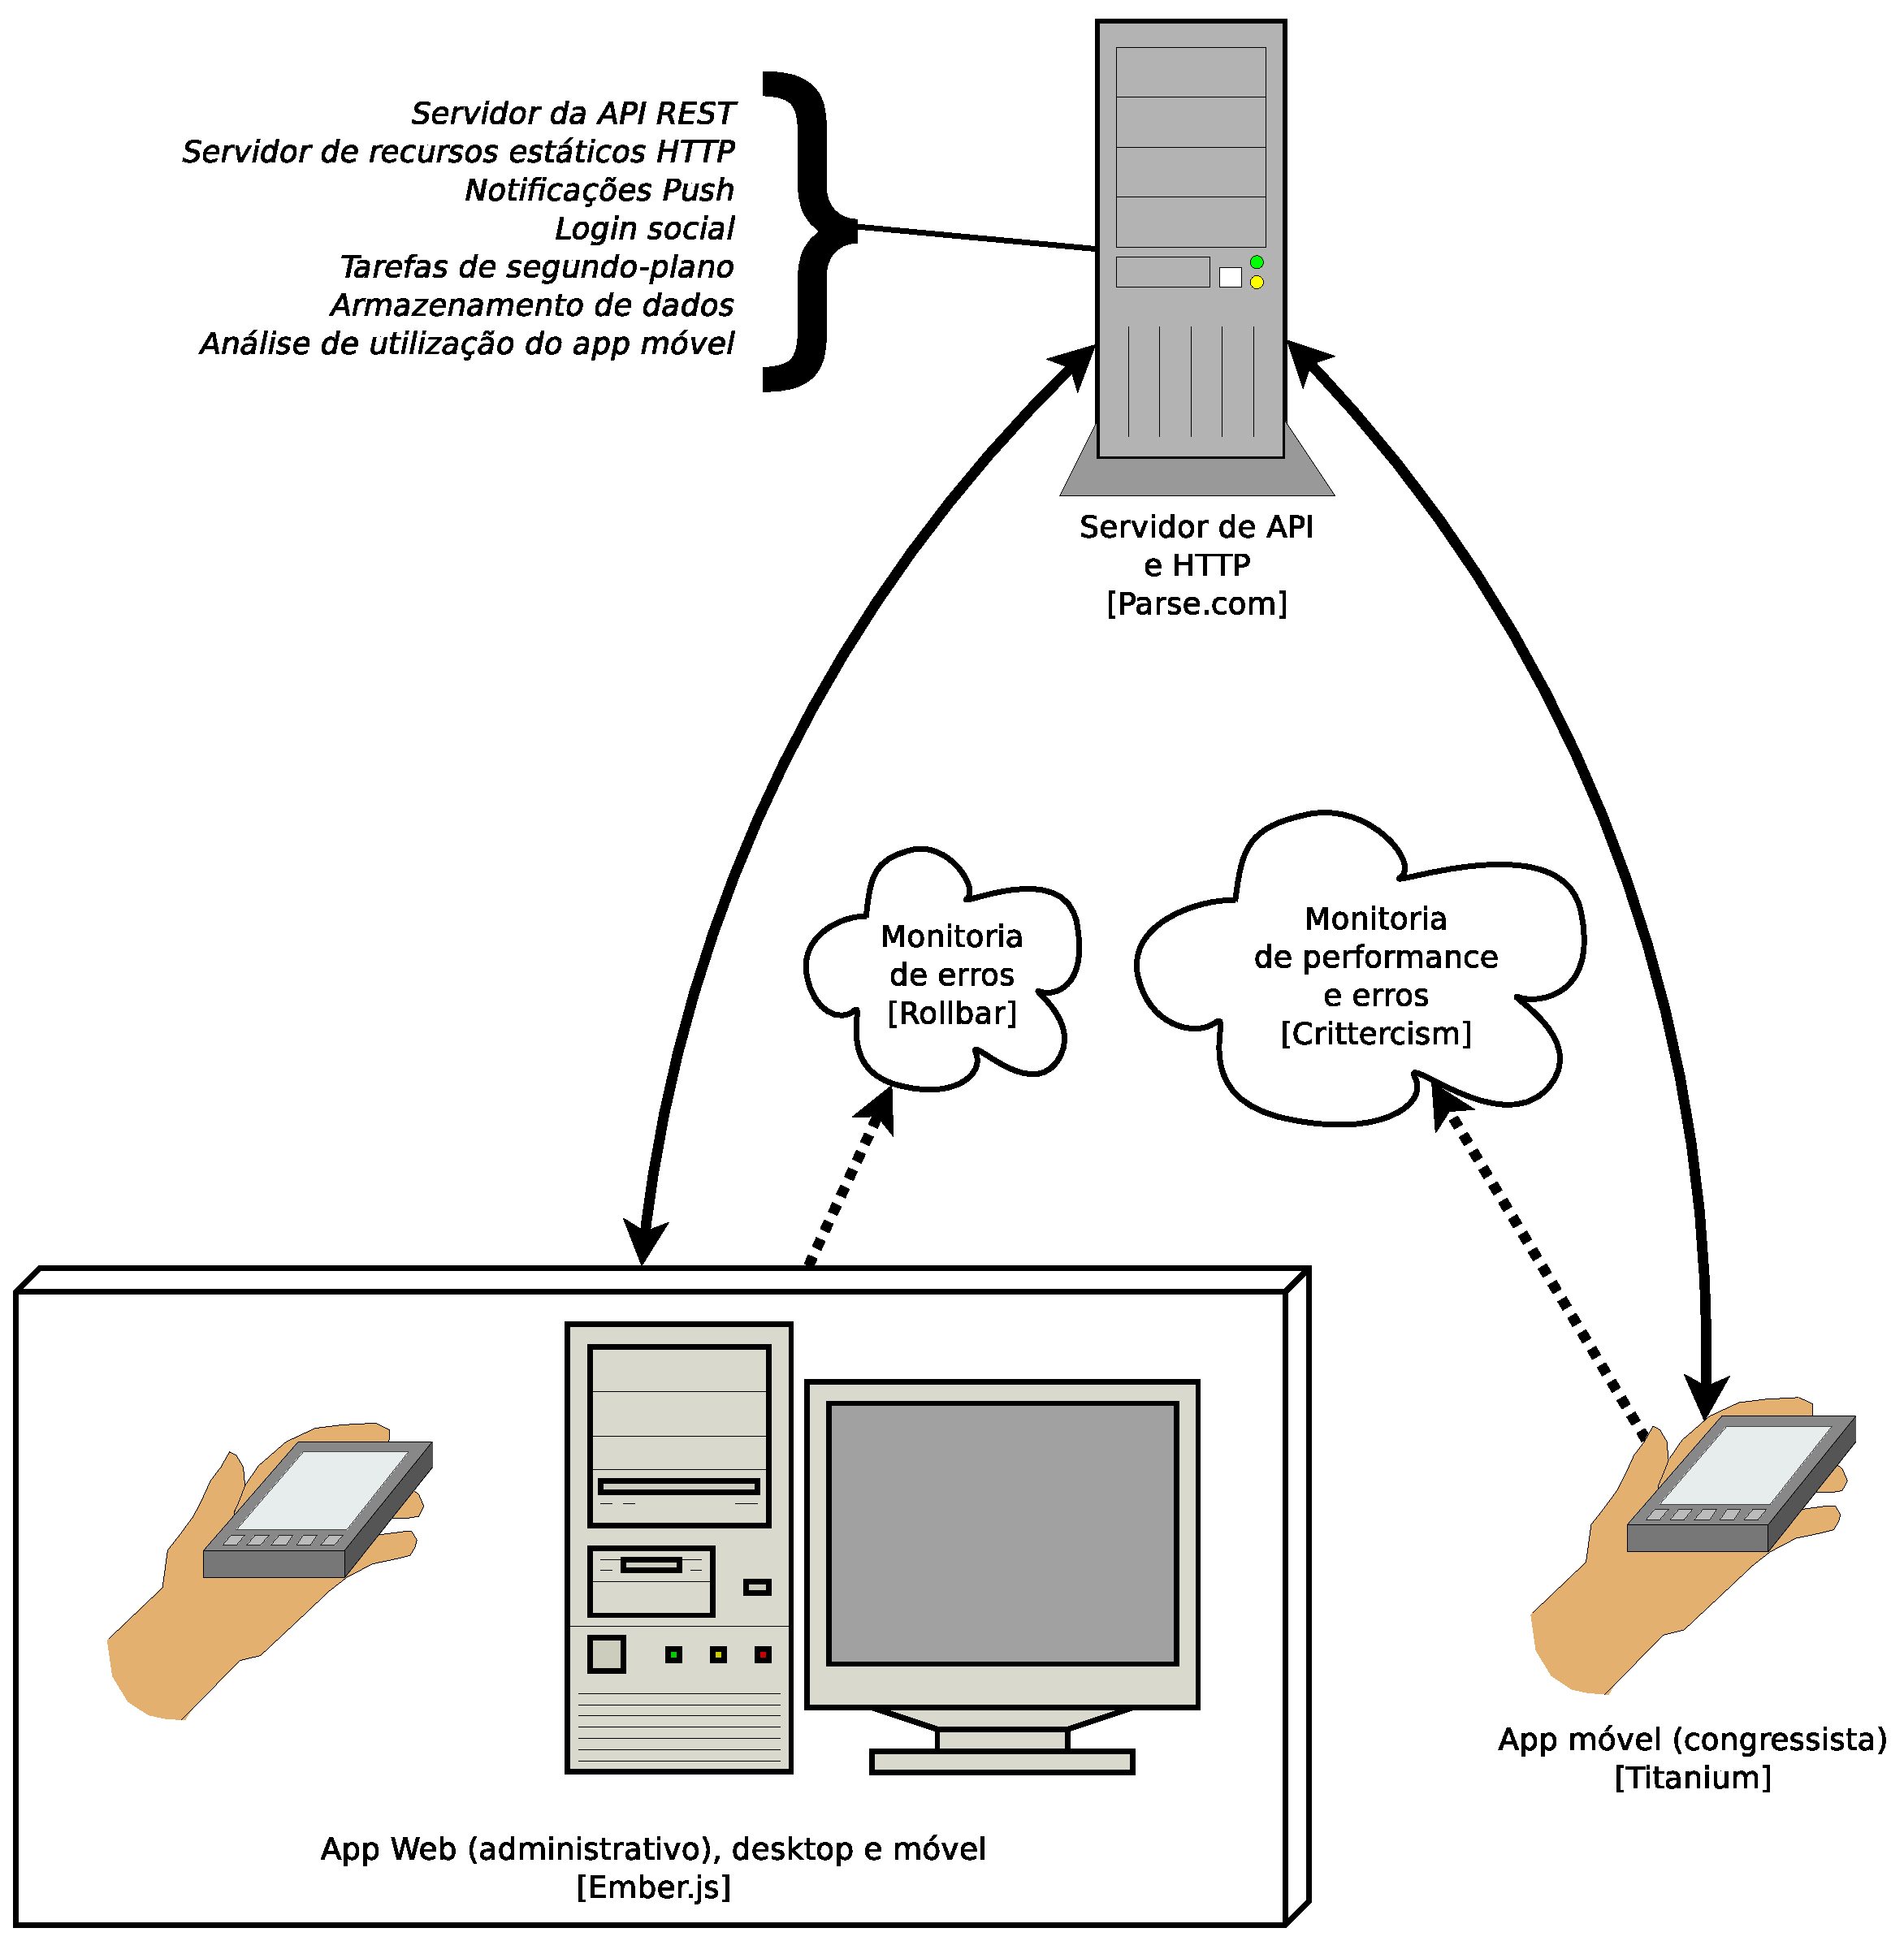
\includegraphics[width=0.8\linewidth]{diagramas/topologia-parse.eps}
	\caption{Diagrama de topologia simples, indicando o uso central dos serviços do Parse}
	\label{fig:topologia-parse}
\end{figure}


%%%%%%%%%%%%%%%%%%%%%%%%%%%%%%%%%%%%%%%%%%%%%%%%%%%%%%%%%%%%%%%%%%%%%%%%%%%%%%%%%%%%%%%%%
\printbibliography

\end{document}
